% !TeX root = ../defense.tex

\section{Gravitational Waves}
\frame{\sectionpage}

\begin{frame}{Where do the gravitational waves come from?}
\begin{columns}
\begin{column}{.4\linewidth}
Einstein Equations:
\begin{align*}
	\uncover<+->{
		G_{\mu\nu} &= \frac{8 \pi G}{c^4} T_{\mu\nu}\\
	}
	\uncover<+->{
		G_{\mu\nu} &= G_{\mu\nu} (g_{\mu\nu}, \dot{g}_{\mu\nu}, \ddot{g}_{\mu\nu}) \\
		\uncover<+->{&= R_{\mu\nu} - \frac{1}{2} g_{\mu\nu} R}
	}
\end{align*}
\begin{align*}
	\uncover<+->{
		&R = g^{\mu\nu} R_{\mu\nu}\\ 
	}
	\uncover<+->{
		&R_{\mu\nu} = R^{\sigma}_{~\mu\sigma\nu}\\
	}
	\uncover<+->{
		&R^{\sigma}_{~\mu\rho\nu} = {R^{\sigma}}_{\mu\rho\nu} (\dot{g}_{\mu\nu}, \ddot{g}_{\mu\nu})
	}
\end{align*}
\vspace*{\fill}
\end{column}
\hspace*{\fill}
\begin{column}{.4\linewidth}
\uncover<+->{Einstein Field Equations:}
\begin{align*}
	\uncover<+->{
		\text{}
		&G_{\mu\nu} = 0
	}
\end{align*}
\begin{align*}
	\uncover<+->{
		\text{if:\quad}
		&g_{\mu\nu} = \eta_{\mu\nu} \text{\quad(everywhere)}\\
	}
	\uncover<+->{
		\therefore\quad &R_{\mu\nu} = 0 \implies G_{\mu\nu} = 0
	}
\end{align*}
\uncover<+->{First order variations:}
\begin{align*}
	\uncover<+->{
		\text{if:\quad}
		g_{\mu\nu} &= \eta_{\mu\nu} + \varepsilon h_{\mu\nu}\\
	}
	\uncover<+->{
		&~~\vdots \\
	}
	\uncover<+->{
		\therefore \quad \Aboxed{\Box h_{\mu\nu} &= 0}
	}
\end{align*}
%\vfill
\end{column}
\end{columns}
\end{frame}

\begin{frame}{But what are gravitational waves?}
\begin{columns}
\begin{column}{0.5\linewidth}
\begin{align*}
	\uncover<+->{
		&\Box h_{\mu\nu} = 0 \\~\\
		\uncover<+->{\rightarrow \quad &\frac{1}{c^2}\frac{\partial^2}{\partial t^2}h_A = \left(\frac{\partial^2}{\partial x^2} + \frac{\partial^2}{\partial y^2} + \frac{\partial^2}{\partial z^2} \right) h_A\\
		&\scriptstyle{(T = +, \times)}}\\
	}
\end{align*}
\uncover<4->{In Transverse-Traceless Guage:}\\
\begin{align*}
	\uncover<5->{
		h_{\mu\nu} = 
		\begin{pmatrix}
			0  & 0         & 0         & 0 \\
			0  & h_+       & h_\times  & 0  \\
			0  & h_\times  & -h_+      & 0  \\
			0  & 0         & 0         & 0 
		\end{pmatrix}
	}
\end{align*}
\end{column}
\begin{column}{0.5\linewidth}
\vfill
\uncover<3->{
	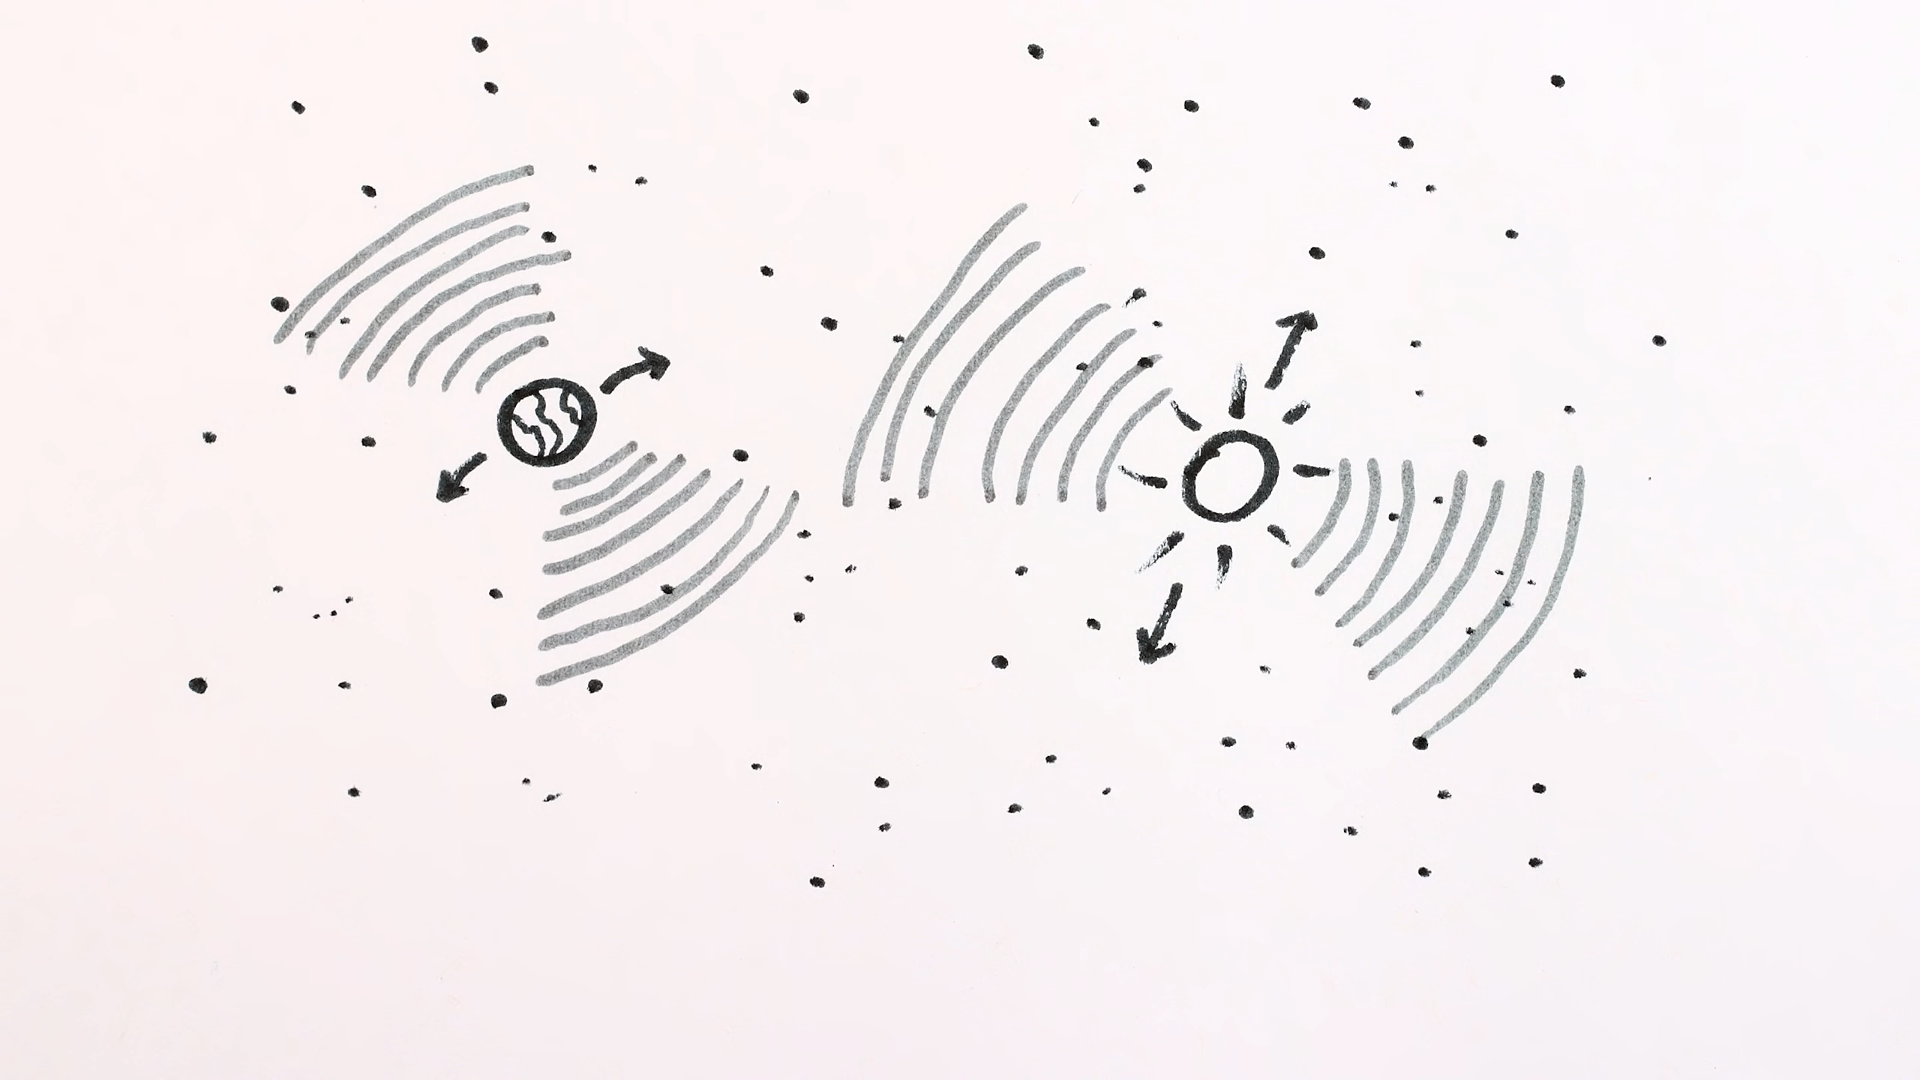
\includegraphics[width=\linewidth]{img/GW-minutephysics}
	\textcolor{gray}{\fontsize{7.5}{10}\selectfont Image credit: \href{https://www.youtube.com/channel/UCUHW94eEFW7hkUMVaZz4eDg}{Youtube: minutephysics}}
}
\end{column}
\end{columns}
\end{frame}

\begin{frame}{Polarizations are the signature of gravitational waves}
\begin{columns}
\begin{column}{.7\linewidth}
	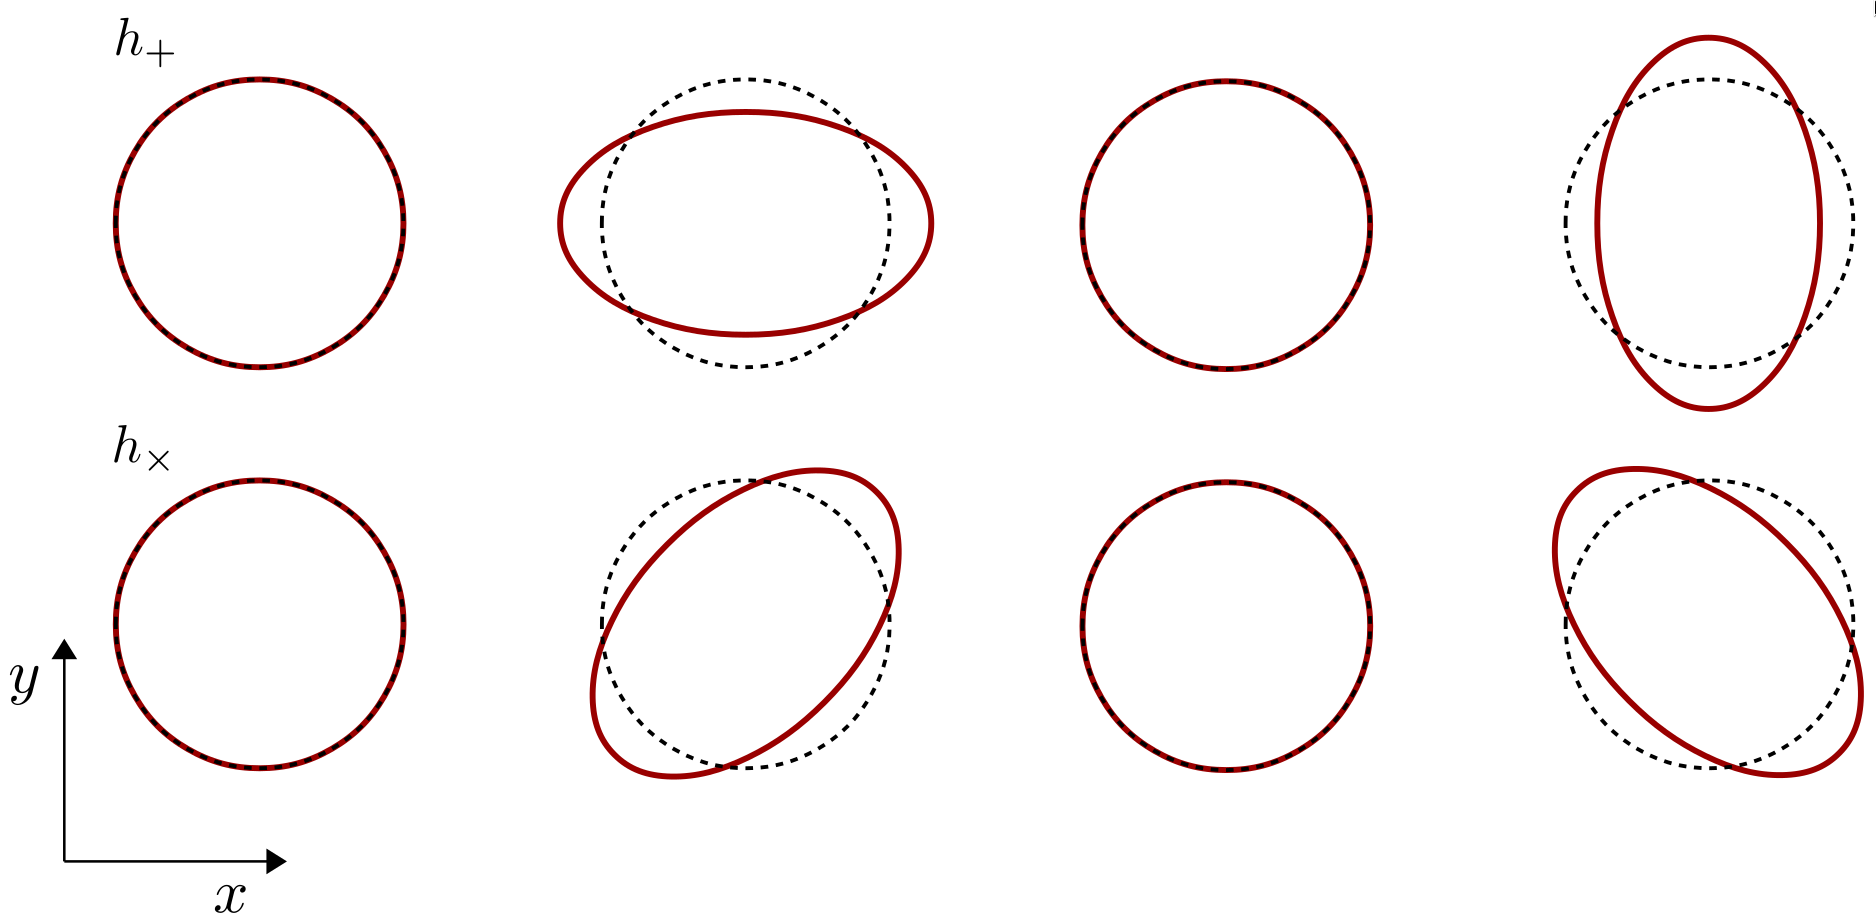
\includegraphics[width=\linewidth]{img/polarization}
\end{column}
\begin{column}{.3\linewidth}
	\textcolor{gray}{\fontsize{7.5}{10}\selectfont Image credit:\\ \href{https://www.elsevier.com/books/modern-cosmology/dodelson/978-0-12-815948-4}{S. Dodelson, F. Schmidt, Modern Cosmology}}
	\vspace*{\fill}
\end{column}
\end{columns}
\vspace*{\fill}
\uncover<2->{Other Gravitational wave features:\\}
\begin{itemize}
	\item<3-> They can not be detected locally (Because of equivalance principal)
	\item<4-> They travel at the speed of light
\end{itemize}
\end{frame}


\begin{frame}{Sources of Gravitational Waves}
\begin{columns}
\begin{column}{.6\linewidth}
\uncover<+->{Burst:}
\begin{itemize}
	\item<+-> Supernovae \\~\\
\end{itemize}
\uncover<4->{Continuous and Inspiral:}
\begin{itemize}
	\item<5-> Binary mergers (NS, SBH, PBH, SMBH, ...)
	\item<6-> Neutron stars with deformities \\~\\
\end{itemize}
\uncover<8->{Stochastic:}
\begin{itemize}[<9->]
	\item<9-> Primordial tensor perturbations
	\item<10-> Secondary tensor perturbations
	\item<11-> Topological defects (e.g. cosmic strings)
	\item<12-> Superposition of the other types
\end{itemize}
\end{column}
\begin{column}{.4\linewidth}
\uncover<3->{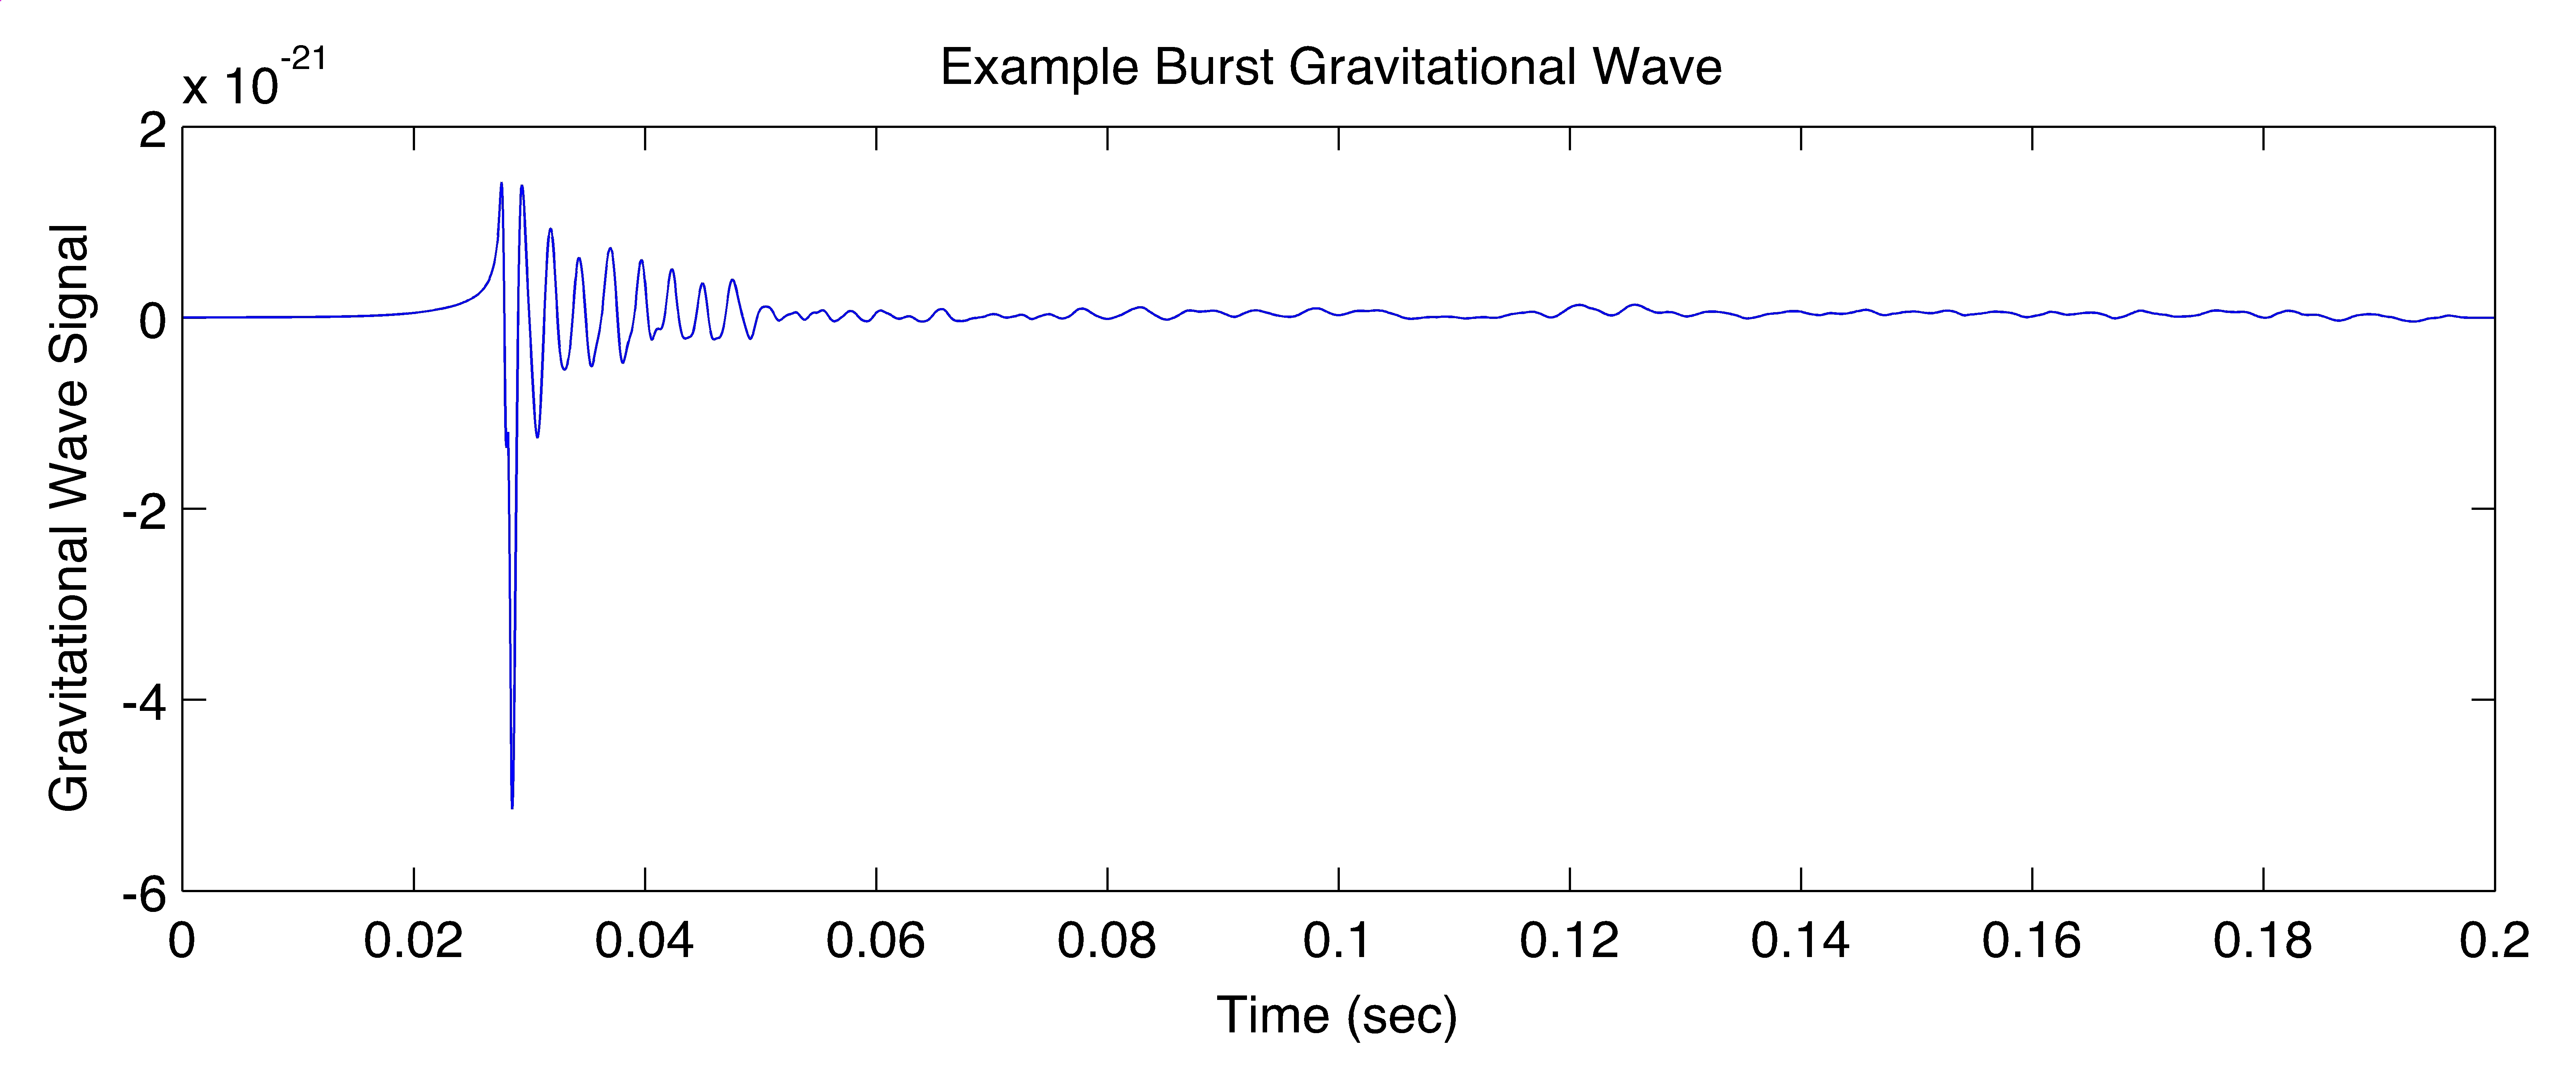
\includegraphics[width=\linewidth]{img/burst}}
\uncover<7->{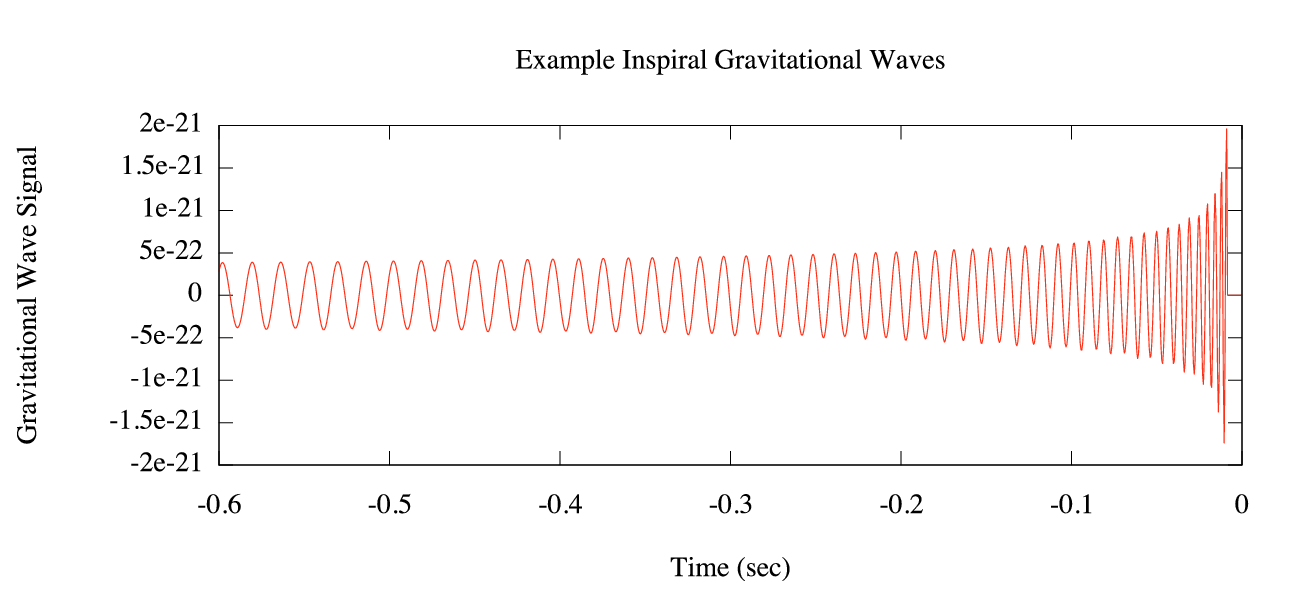
\includegraphics[width=\linewidth]{img/inspiral-0}}
\uncover<13->{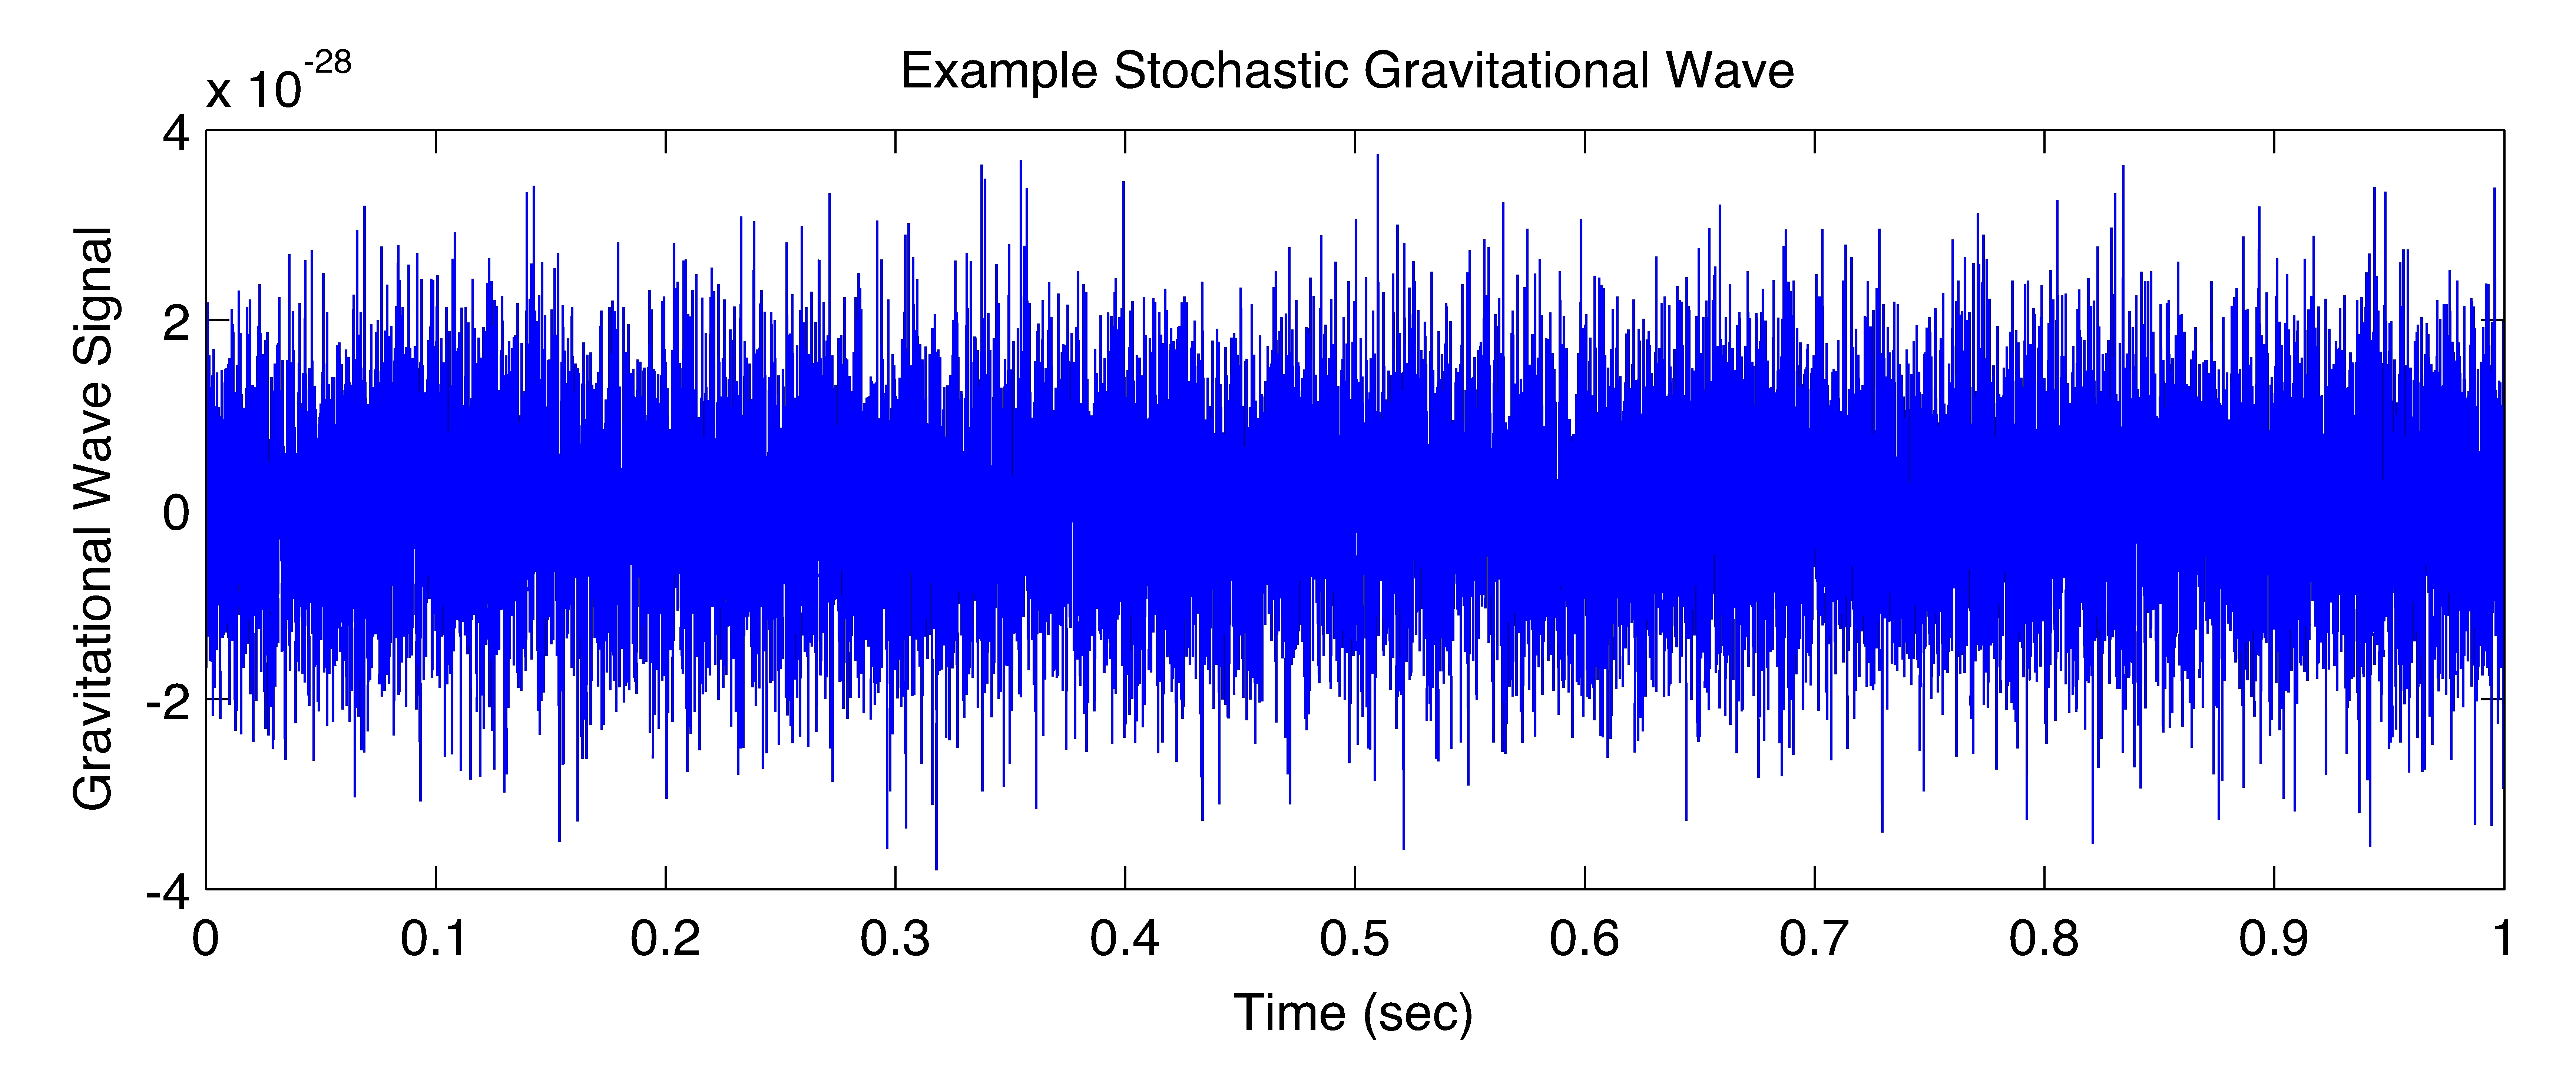
\includegraphics[width=\linewidth]{img/stochastic}}
\uncover<3->{
	\textcolor{gray}{\fontsize{4.5}{10}\selectfont Image credit:
	\href{https://www.ligo.org/science}{LIGO Scientific Collaboration}}
}
\end{column}
\end{columns}
\end{frame}

\begin{frame}{How to detect gravitational waves?}
\begin{columns}
\begin{column}{0.63\linewidth}
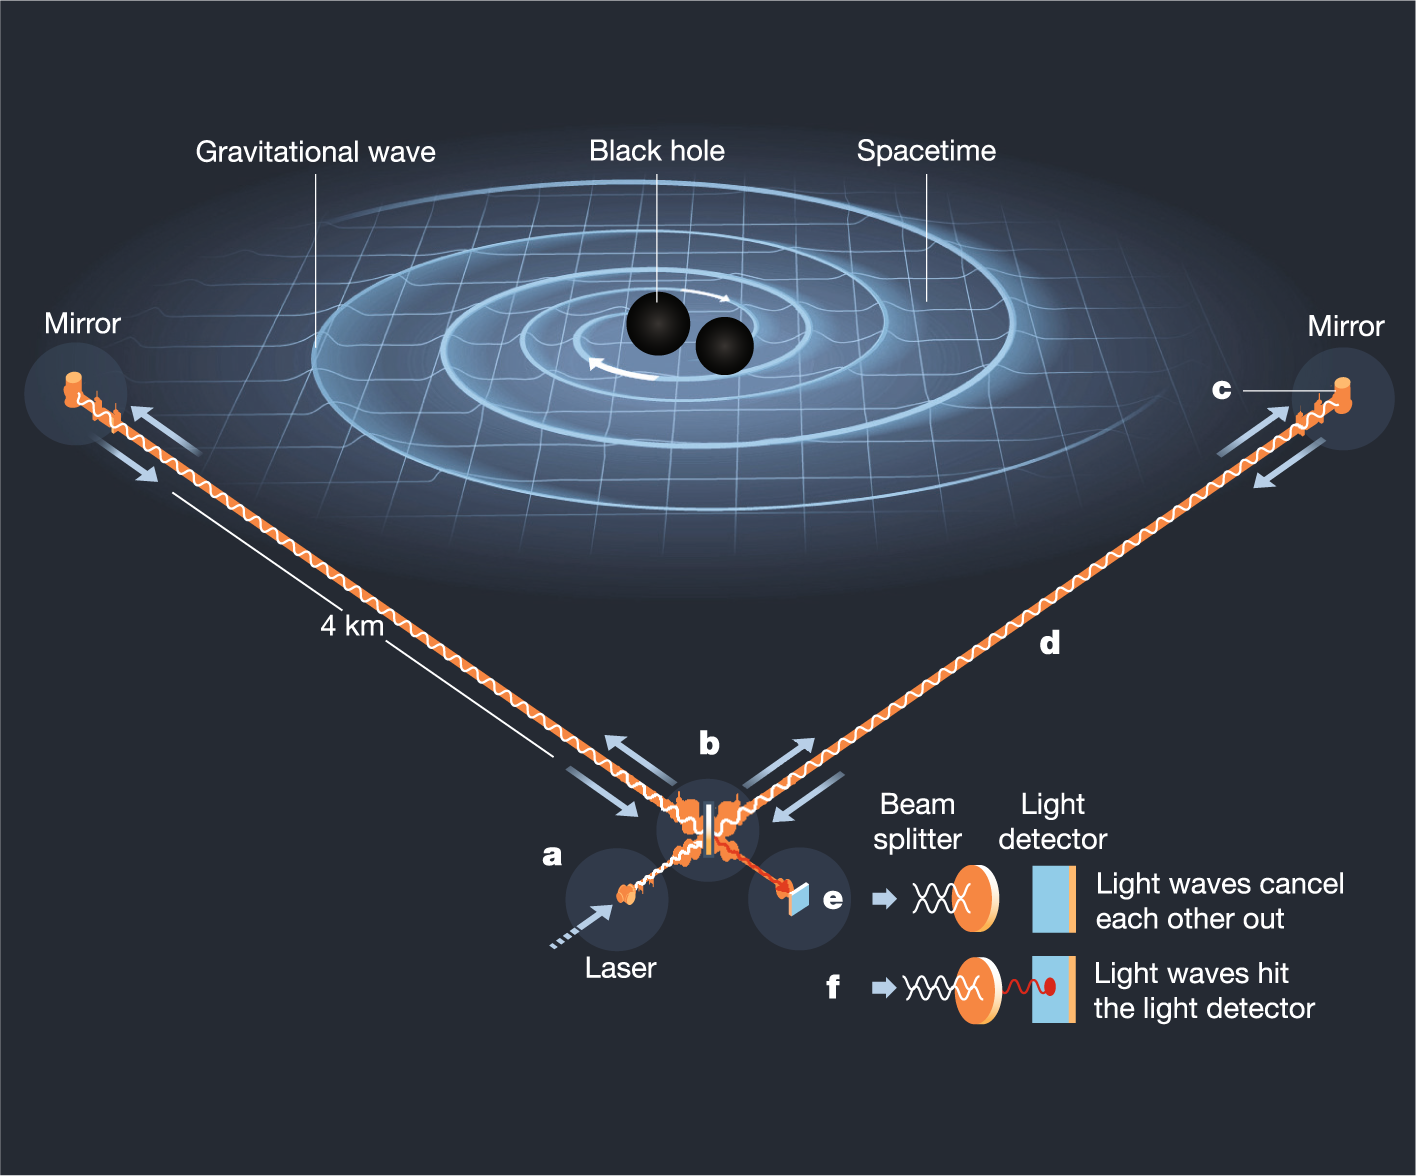
\includegraphics[width=\linewidth]{img/LIGO_setup}
\end{column}
\begin{column}{0.32\linewidth}
	\uncover<2->{
		Other detection methods:
	}
	\begin{itemize}
		\item<3-> Weber bar
		\item<4-> Pulsar timing arrays
		\item<5-> CMB B-mode
		\item<6-> Other non-direct ways
	\end{itemize}
	\vspace*{4cm}
	\textcolor{gray}{\fontsize{7.5}{10}\selectfont Image credit:
	\href{https://www.nobelprize.org/prizes/physics/2017/press-release/}{The Royal Swedish Academy of Sciences}}
\end{column}
\end{columns}
\end{frame}

\begin{frame}{Gravitational waves from black hole mergers}
\vskip 5pt
\centering
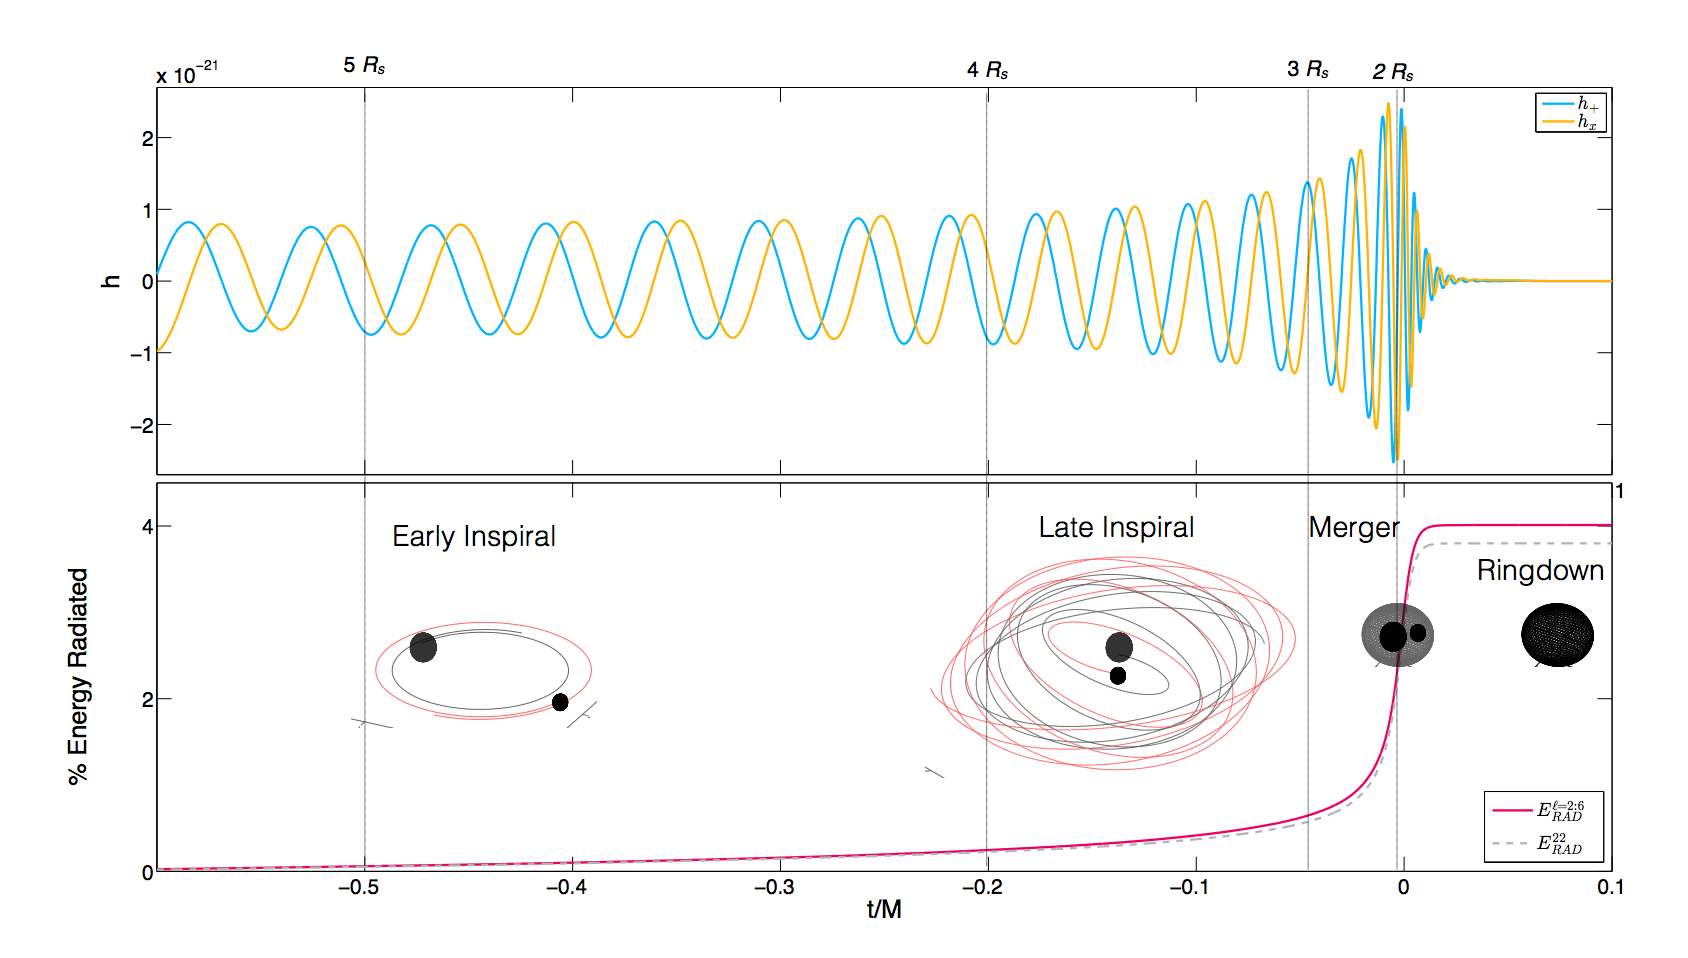
\includegraphics[width=\linewidth]{img/BBH_GT}\\
\vskip -10pt
\qquad\qquad\qquad\qquad\qquad\qquad\qquad\qquad\qquad\qquad\textcolor{gray}{\fontsize{7.5}{10}\selectfont Image credit:
\href{https://einstein.gatech.edu/catalog/}{Einstein at Georgia Tech}}
\end{frame}

\begin{frame}{Stochastic gravitational wave background}
\begin{columns}
\begin{column}{0.5\linewidth}
	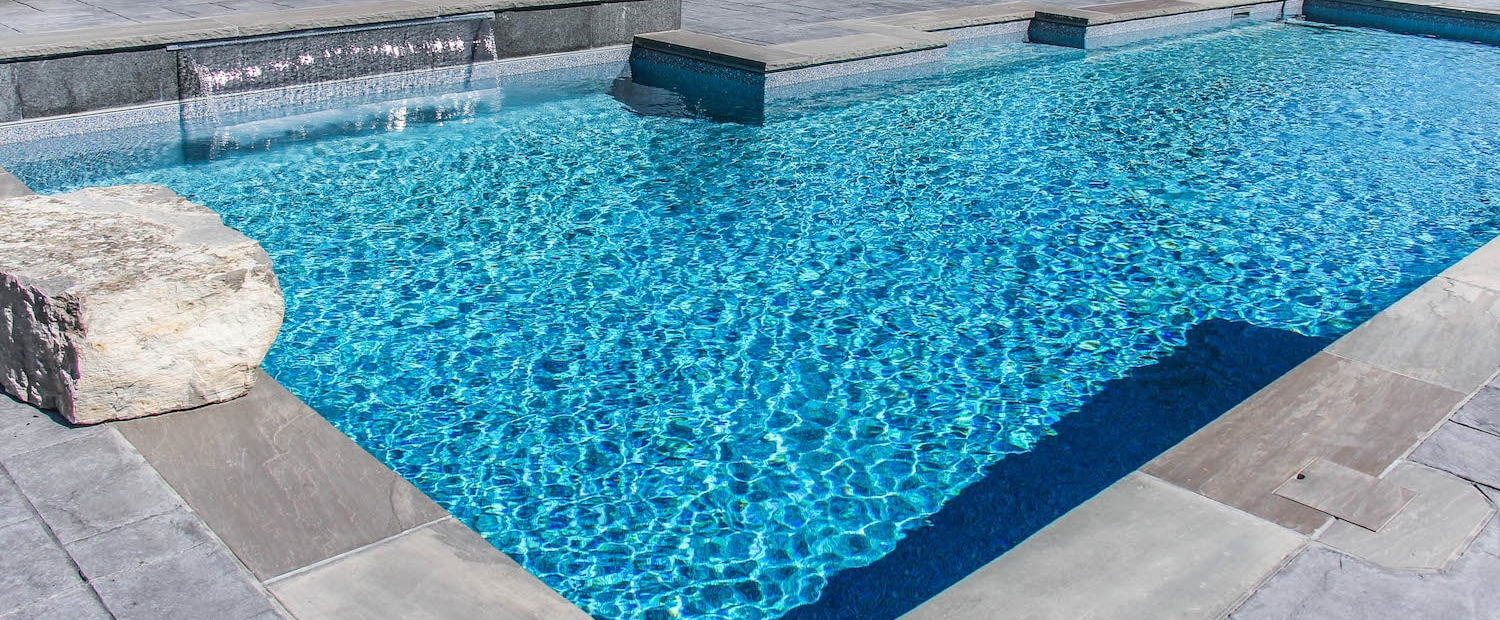
\includegraphics[width=\linewidth]{img/pool}
	\textcolor{gray}{\fontsize{6.5}{10}\selectfont Image credit: \href{http://www.megnapools.com/aqua-blue-mixnmatch}{Megna pools}}
\end{column}
\begin{column}{0.5\linewidth}
"We are like an insect sitting at the edge of a pool, trying to figure out who jumped in where and when and what's happening all over the pool."\\~\\
- Richard Feynman
\hfil
\end{column}
\end{columns}
\begin{columns}
\begin{column}{.55\linewidth}
\begin{align*}
	\uncover<2->{
		&\Omega_{SGWB} (f) = \frac{1}{\rho_c} \frac{\der \rho_{GW}(f)}{\der \ln f}\\~\\
	}
	\uncover<3->{
		h_{ab} &(t, \vec{x})\\&= \sum_{A=+,\times} \int_{-\infty}^{\infty} \der f \int_{S^2} \der \hat{\Omega} h_A(f, \hat{\Omega}) e^{2\pi i f (t - \hat{\Omega} \cdot \vec{x})} \hat{e}_{ab}^A (\hat{\Omega})
	}
\end{align*}
\end{column}
\begin{column}{.45\linewidth}
\begin{align*}
\uncover<4->{
	\langle h_A(f, \hat{\Omega})& h^*_{A^\prime}(f^\prime, \hat{\Omega}^\prime) \rangle_{\text{ens}}\\ &=\frac{\delta_{AA^\prime}}{2} \frac{\delta^{(2)} (\hat{\Omega}, \hat{\Omega}^\prime)}{4\pi} \frac{\delta(f - f^\prime)}{2} S_h(f)\\~\\
}
\uncover<5->{
	\Aboxed{&\Omega_{SGWB} (f) = \frac{2 \pi^2 c^4}{3 H_0^2} f^3 S_h(f)}
}
\end{align*}
\end{column}
\end{columns}
\end{frame}

\begin{frame}{Recap}
\uncover<+->{We want to detect:}
\begin{itemize}[<+->]
	\item A stochastic gravitational wave background
	\item Coming from binary black hole mergers
	\item Our chosen black holes to study have a primordial origin
\end{itemize}
\vskip 1cm
\uncover<+->{To achieve these, we need:}
\begin{enumerate}[<+->]
	\item Learn about primordial black holes and their population statistics
	\item Build a model for their merger rates based on the population statistics
	\item Simulate a stochastic gravitational wave background
	\item Build a model to analyse the data
	\item Run the analyses
\end{enumerate}
\end{frame}